% subseccion 4.1  
\subsection{Planeación}
En esta etapa, se estableció el proposito general de la investigación y se definieron las metas, así como las preguntas de investigación, métricas, criterios de clasificación, criterios de inclusión/exclusión y criterios de calidad de los estudios.
Ver Figura\ref{fig:etapa1}.

\begin{figure*}[htbp]
    \centering
    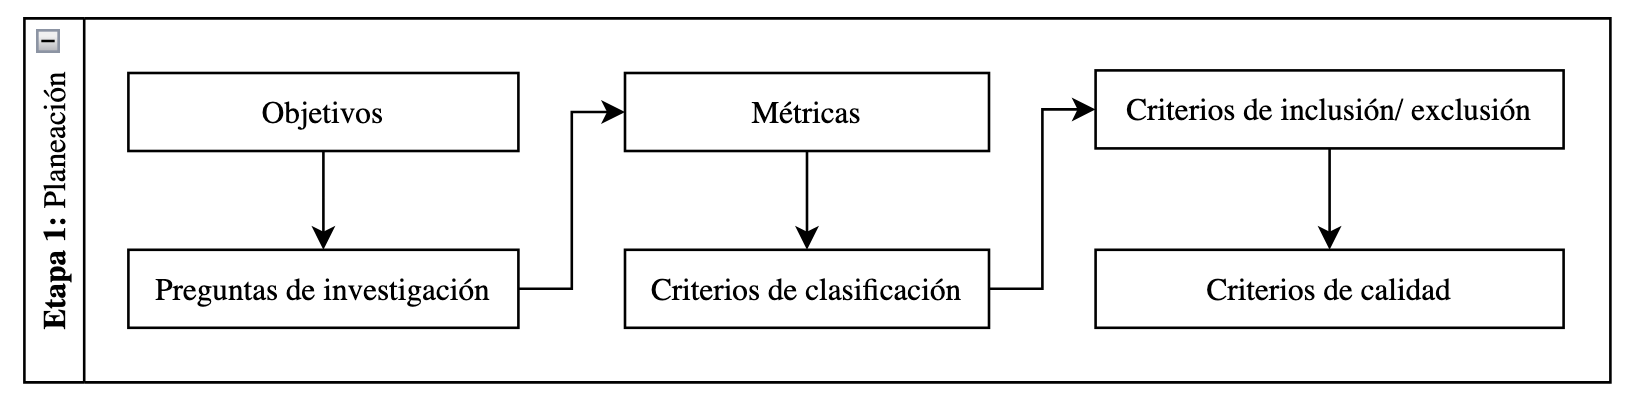
\includegraphics[width=0.8\textwidth]{resources/images/planeacion/etapa1.png}
    \caption{Composición de la etapa de planeación}\label{fig:etapa1}
\end{figure*}


% 4.1.1
%sub-subseccion - objetivos del estudio
\subsubsection{Objetivos}
\mbox{}\\
Teniendo en cuenta los aspectos descritos en la sección de motivación, se definieron 2 metas generales para la revisión sistemática de la literatura que se presentan en la Tabla \ref{tab:metas}.

\begin{table}[H]
    \centering
    \begin{tabular}{>{\centering\arraybackslash}m{1cm}>{\arraybackslash}m{7cm}}
        \hline
        \textbf{Goal} & \textbf{Description} \\
        \hline
        \\
        M1 & Identificar trabajos relacionados con VBC en proyectos de docencia, investigación y extensión. \\
        \\
        M2 & Clasificar trabajos relacionados con VBC en los dominios de desarrollo de software, pensamiento computacional, computación paralela, análisis de datos, inteligencia artificial, redes computacionales, infraestructura de TI, HPC, entre otros. \\
        \\
        \hline
    \end{tabular}
    \caption{Metas del estudio}\label{tab:metas}
\end{table}


% 4.1.2
%sub-subseccion - pregunta de investigación
\subsubsection{Pregunta de investigación}
\mbox{}\\

% 4.1.3
%sub-subseccion - metricas
\subsubsection{Métricas}
\mbox{}\\

% 4.1.4
%sub-subseccion - topicos de investigación
\subsubsection{Tópicos de investigación}
\mbox{}\\

% 4.1.5
%sub-subseccion - criterios de inclusión y exclusión
\subsubsection{Criterios de inclusión y exclusión}
\mbox{}\\

% 4.1.6
% sub-subseccion - Criterios de calidad
\subsubsection{Criterios de calidad}
\mbox{}\\
